%!TEX root = ../../novoIndex.tex
Levando em conta a adoção de CNNs como o modelo de ML a ser usado neste trabalho, considerou-se inicialmente a utilização das arquiteturas LeNet e AlexNet. A implementação da AlexNet, em particular, seguiu a prática de utilizar apenas uma GPU em seu treinamento, segundo a qual as camadas ora paralelas no trabalho original foram unificadas de forma sequencial \cite{tensorflow:alexnet}. Adotou-se um \emph{batch size} igual a $64$ para o treinamento, e o método de otimização do gradiente descendente foi o \emph{Adam}. O número de épocas foi obtido de maneira experimental e a taxa de aprendizado é adaptativa, sendo iniciada com $10^{-3}$ e com decaimento suave de $10^{10}$, observando a perda obtida ao final de cada época.

Além da LeNet e AlexNet, duas redes mais profundas foram aplicadas para a tarefa: a VGG-16 e a SqueezeNet. A arquitetura profunda VGG-16 foi utilizada em uma tarefa de estimação de idade previamente descrita na literatura obtendo resultados satisfatórios, conforme Seção \ref{sec:trab_relac} e  \cite{rothe2015dex}. A SqueezeNet, por sua vez, é uma CNN proposta recentemente na literatura, datada de 2018, especialmente voltada para os mesmos cenários da AlexNet, prometendo o mesmo desempenho, mas com 50 vezes menos parâmetros \cite{squeezenet}. No contexto de uma aplicação em que se necessita prover ao usuário respostas rápidas obtidas em \emph{hardware} limitado, tal como ocorre neste cenário em que se consideram as \emph{Smart TVs}, o potencial das características positivas destas redes torna propícia a investigação de sua adequação. O número de épocas de treinamento e a taxa de aprendizado inicial seguiram as mesmas práticas e valores daqueles adotados na LeNet e AlexNet.

É importante ressaltar que as quatro arquiteturas de CNNs consideradas, LeNet, AlexNet, VGG-16 e SqueezeNet, foram originalmente propostas para problemas de classificação, entretanto, no contexto deste trabalho, considera-se um problema de regressão. A fim de promover esta adaptação, a camada de saída, que anteriormente era constituída de múltiplos neurônios sujeitos à função de ativação \emph{softmax}, foi substituída por um único neurônio. Considerou-se utilizar duas funções de ativação distintas na saída deste neurônio: a função \emph{ReLU}, previamente apresentada na Seção \ref{sec:rnas}, e também a função \emph{Leaky ReLU}, e expressa na Figura \ref{fig:lrelu}. Esta última visa contornar um problema de estagnação típico durante o treinamento de CNNs com  função de ativação \emph{ReLU}, o chamado \emph{dying ReLU problem}, tendo como características ser diferenciável e monotônica, colaborando também para a introdução de não-linearidade.


\begin{figure}[!ht]
     \centering
     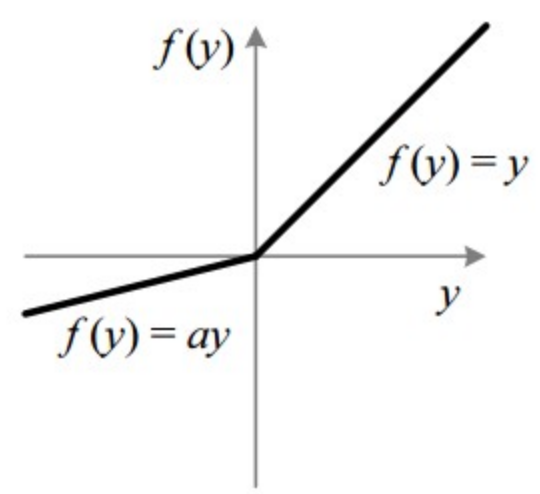
\includegraphics[width=0.3\textwidth]{img/lrelu}
     \caption{Função de Ativação \emph{Leaky ReLU}}
     \label{fig:lrelu}
\end{figure}

Definidos os parâmetros relativos às arquiteturas das CNNs e de suas funções de ativação, bem como os hiperparâmetros relativos ao treinamento no que diz respeito ao número de épocas, taxa de aprendizado e otimizador, partiu-se então para, enfim, o treino e teste dos modelos propostos, cujos resultados são discutidos no capítulo a seguir.
